\chapter{XÁC ĐỊNH VẤN ĐỀ NGHIÊN CỨU}
\label{Chapter1}

\section{Tính cấp thiết của đề tài}

Ra mắt lần đầu vào năm 2005 và có mặt chính thức tại Việt Nam từ năm 2014, YouTube giờ đây không chỉ là một nền tảng chia sẻ video, mà đã trở thành một kho dữ liệu khổng lồ, mang lại giá trị khai thác cho nhiều lĩnh vực ngành nghề. Theo nghiên cứu của \textcite{choudhury_2019}, Việt Nam hiện nằm trong nhóm 5 thị trường chiến lược hàng đầu, thu hút lượng đầu tư mạnh mẽ bậc nhất từ nền tảng này trên quy mô toàn cầu. Số liệu thống kê từ DataReportal \parencite{kemp_2026} tính đến cuối năm 2025 cũng cho thấy YouTube đang sở hữu tới 62,1 triệu người dùng tại Việt Nam, chiếm 61\% dân số cả nước. Cùng lúc đó, báo cáo của Decision Lab \parencite{decision_lab_2025} ghi nhận tỷ lệ thâm nhập của nền tảng này đạt 87\% trong quý IV/2025 (Hình~\ref{fig:ti_le_tham_nhap}), chỉ đứng sau Facebook, Zalo và bỏ xa TikTok. Những con số này cho thấy hệ sinh thái YouTube đang đường cho các bài toán giám sát thông tin mạng xã hội trực tuyến (Social Media Listening), tức quá trình vận dụng khai thác dữ liệu tiên tiến nhằm theo dõi, chắt lọc thông tin có giá trị từ những cuộc trò chuyện, thảo luận xoay quanh một chủ đề nhất định trên mạng xã hội (chẳng hạn một thương hiệu hay hashtag), qua đó hỗ trợ phát hiện cơ hội kinh doanh, tối ưu hoạt động tiếp thị và nâng cao chất lượng phục vụ người tiêu dùng \parencite{ducange_2019}.

\begin{figure}[htbp]
    \centering
    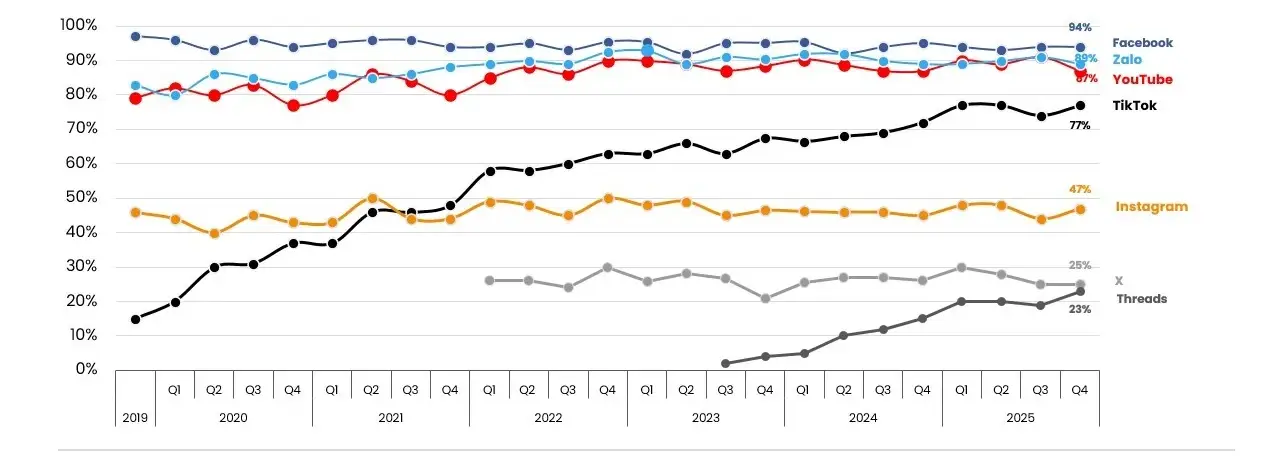
\includegraphics[width=0.8\textwidth]{Images/decision_lab_iv_2025_re.png}
    \caption{Biểu đồ tỷ lệ thâm nhập của các nền tảng mạng xã hội dẫn đầu tại Việt Nam, từ Decision Lab, quý IV 2025}
    \label{fig:ti_le_tham_nhap}
    \vspace{0.1cm}
    {\small Nguồn: \textcite{decision_lab_2025}}
\end{figure}

Những tiến bộ vượt bậc mà \gls{ml} đạt được trong giai đoạn hiện nay đã mở đường cho việc khai thác chuyên sâu các nguồn dữ liệu phi cấu trúc bên cạnh những định dạng có cấu trúc vốn quen thuộc trước đây. Bản thân văn bản là một nguồn tài nguyên thông tin giàu giá trị, lưu giữ các trạng thái nội tâm (private states) của con người như ý kiến, niềm tin, suy nghĩ, tình cảm, cảm xúc, mục tiêu, đánh giá và phán đoán \parencite{wiebe_2005}. Chính vì vậy, việc ứng dụng kỹ thuật \gls{sa} để đo lường mức độ phân cực của ngôn từ là hướng tiếp cận chủ đạo, góp phần nâng cao hiệu quả trích xuất thông tin trên các nền tảng mạng xã hội.

Dù kho dữ liệu công khai trên YouTube có quy mô đồ sộ, đa dạng và mang đặc tính đa miền (multi-domain), các hướng tiếp cận hiện có tại Việt Nam vẫn chưa khai thác hết tiềm năng này và còn tồn tại một số khoảng trống nhất định. Trong khi bài toán nhận diện sắc thái tâm lý trên các ngôn ngữ phổ biến toàn cầu đã đạt được nhiều bước tiến đáng kể \parencite{guo2024mvindemo, zhao2024multi, shen2025zero, zhao2025interpretable, lee2026dimabsa}, thì phần lớn công trình liên quan đến tiếng Việt vẫn bó hẹp trong phạm vi các tập dữ liệu ngách, chỉ giới hạn ở một số miền cụ thể \parencite{minh2024fine, le2025hybrid, nguyen2025like}.

Mặt khác, mặc dù góp mặt trong top 20 ngôn ngữ có cộng đồng người sử dụng đông đảo nhất thế giới \parencite{ethnologue_2026}, tiếng Việt vẫn tiềm ẩn không ít thách thức riêng khi đưa vào xử lý. Trước hết, sự phong phú của các phương ngữ và vốn từ vựng địa phương gây ra không ít trở ngại cho các công cụ xử lý ngôn ngữ tự nhiên (\acrshort{nlp}). Kế đến, sự giao thoa diễn ra trên không gian mạng đã làm cho hiện tượng trộn mã (code-switching) (chẳng hạn: "sản phẩm nhìn rất chill") ngày càng phổ biến và liên tục biến đổi. Thêm vào đó, cách con người diễn đạt cảm xúc luôn thay đổi, cộng với sự xuất hiện của những từ vựng mới, buộc các mô hình ML phải sở hữu khả năng thích nghi cao (adaptability) để không bị suy giảm hiệu năng trước những biến động của ngôn ngữ xã hội.

Đối diện với những thách thức kể trên, các phương pháp cổ điển như hệ thống dựa trên luật (rule-based) hay những kiến trúc mạng học sâu thế hệ trước (\gls{rnn}, \gls{lstm}) dần cho thấy sự hạn chế, bởi chúng thường gặp khó khăn khi phải ghi nhớ thông tin xuyên suốt một chuỗi ngữ cảnh dài và giải mã cấu trúc câu trộn mã phức tạp. Mạng Transformer với cơ chế tự chú ý (Self-Attention) \parencite{vaswani2017attention} giải quyết triệt để rào cản này nhờ khả năng nắm bắt toàn bộ ngữ cảnh văn bản dài mà không phụ thuộc vào khoảng cách, qua đó nâng cao độ chính xác khi xử lý các tác vụ nhận diện thái độ trên dữ liệu đa miền.

Từ những đòi hỏi cấp thiết vừa nêu, câu hỏi được đặt ra là làm thế nào để xây dựng một khung phương pháp (framework) chuẩn hóa, vận dụng kiến trúc Transformer nhằm giải quyết các khó khăn đặc thù của dữ liệu YouTube trong bối cảnh Việt Nam. Đây không chỉ là một bài toán mang giá trị lý luận sâu sắc, mà còn ẩn chứa tiềm năng ứng dụng thực tiễn to lớn. Khung phương pháp được đề xuất sẽ là công cụ hữ-u ích, giúp các nhà sáng tạo nội dung lẫn doanh nghiệp nắm bắt tâm lý khán giả, từ đó có cơ sở vững chắc để hoạch định chiến lược mở rộng nội dung và tối ưu hóa hiệu quả kinh doanh.

\section{Mục tiêu nghiên cứu}

\subsection{Mục tiêu chung}
Xuất phát từ những luận điểm vừa được trình bày, có thể khẳng định rằng xây dựng một khung phương pháp trên nền tảng kiến trúc Transformer, đang trở nên cấp bách, nhằm giải quyết trọn vẹn bài toán nhận diện sắc thái tâm lý của người dùng không chỉ trên YouTube mà còn trên các nền tảng mạng xã hội khác tại Việt Nam. Mục tiêu cốt lõi của khung phương pháp này là tối ưu hóa toàn diện chuỗi công đoạn thiết lập và triển khai vào thực tế, từ việc thu thập dữ liệu trên môi trường internet, tiền xử lý dữ liệu đầu vào, cơ chế gắn nhãn tự động, cho tới khâu mô hình hóa theo hướng bám sát các xu thế công nghệ hiện đại.

Dựa trên thang đo tâm lý mà \textcite{demszky2020goemotions} dựng lên từ cơ sở thực nghiệm của \textcite{cowen2019primacy}, nghiên cứu này hướng đến việc bóc tách và làm rõ tính phức tạp, đa chiều trong trạng thái tâm lý con người thông qua 27 phạm trù cảm xúc vi mô có độ hạt mịn (fine-grained), một bước tiến xa hơn so với hệ thống phân loại sáu lớp cơ bản của \textcite{ekman1992there} hay các cách đánh giá phân cực thô sơ trước đây. Đặc biệt, bằng việc thiết lập bài toán theo hướng phân loại đơn nhãn độc lập, nghiên cứu không hề phủ nhận tính liên tục vốn có của không gian cảm xúc; thay vào đó, trọng tâm được đặt vào việc xây dựng một cơ chế lọc thông tin hiệu quả nhằm xác định chính xác luồng tâm lý chủ đạo (dominant emotion) chi phối mạnh nhất trong mỗi phát ngôn. Nhờ vậy, cách tiếp cận này vừa tận dụng được mật độ thông tin phong phú từ những khám phá tâm lý học hiện đại, vừa đảm bảo tính dứt khoát, rõ ràng cần thiết cho các ứng dụng thực tế ở hạ nguồn trên mạng xã hội nói chung và YouTube nói riêng.

\subsection{Mục tiêu cụ thể}
Để hiện thực hóa định hướng tổng thể đã đề ra, đề án xác định bốn mục tiêu cụ thể, được phân bổ theo trình tự của một quy trình hoàn chỉnh bắt đầu từ khâu thu thập, tổ chức dữ liệu cho đến việc mô hình hóa bằng thuật toán phân lớp với nội dung chi tiết như sau:
\begin{itemize}[label=-]
    \item Xây dựng một kho ngữ liệu quy mô lớn từ việc thu thập và tổng hợp các bình luận (comments) cùng siêu dữ liệu (metadata) liên quan đến video trên YouTube; song song đó, thiết lập quy trình tiền xử lý văn bản để bóc tách và chuẩn hóa các đặc trưng phi cấu trúc, bám sát tiêu chuẩn huấn luyện hiện đại của các mô hình ngôn ngữ lớn trong lĩnh vực \acrshort{nlp}, nhằm khử nhiễu đặc thù của ngôn ngữ mạng trong khi vẫn giữ trọn sắc thái ngữ nghĩa ẩn trong từng ký tự và hành vi tương tác.
    \item Vận dụng lược đồ gồm 27 trạng thái cảm xúc cùng một nhãn trung tính (neutral) do \textcite{demszky2020goemotions} đề xuất, kết hợp cơ chế gán nhãn bán tự động với sự phối hợp giữa chuyên gia và mô hình ngôn ngữ quy mô lớn (LLM-Human-in-the-loop), nhằm xác định chuẩn xác cảm xúc chủ đạo (dominant emotion) hiện diện trong từng văn bản theo cách tối ưu, phù hợp bối cảnh hiện nay.
    \item Thực hiện tinh chỉnh (fine-tuning) các thuật toán học sâu dựa trên bộ khung Transformer đã được tiền huấn luyện chuyên biệt cho tiếng Việt, dù đơn ngữ hay đa ngữ (mBERT, PhoBERT, mModernBERT). Đồng thời áp dụng các kỹ thuật xử lý tình trạng chênh lệch tỷ lệ giữa các nhãn (class imbalance) vốn là đặc trưng của dữ liệu thực tế, trước khi đánh giá chặt chẽ độ ổn định và khả năng khái quát hóa của mô hình thông qua các chỉ số thống kê tiêu chuẩn.
    \item Trên các số liệu thực nghiệm thu thập được, hoàn thiện một quy trình (pipeline) chuẩn hóa có năng lực nhận diện chuẩn xác độ phức tạp trong trạng thái tâm lý người dùng đóng vai trò như một nền tảng kỹ thuật hỗ trợ đắc lực cho giới nghiên cứu thông tin xã hội tại Việt Nam, đồng thời mở đường cho các bài toán ứng dụng ở hạ nguồn (downstream tasks) như nắm bắt thị hiếu, đánh giá sức mạnh thương hiệu, hay kiểm soát và xử lý khủng hoảng truyền thông, được vận hành theo hướng tự động hóa, minh bạch, chuyên sâu và tối ưu chi phí.
\end{itemize}

\subsection{Đối tượng nghiên cứu}
\begin{itemize}[label=-]
    \item \textbf{Về mặt dữ liệu và ngôn ngữ học:} Đối tượng khảo sát tập trung vào các biến động tâm lý, thái độ và sắc thái tình cảm đa chiều của người dùng Việt Nam, được thể hiện thông qua ngữ liệu văn bản phi cấu trúc trên nền tảng YouTube.
    \item \textbf{Về mặt công nghệ và thuật toán:} Trọng tâm nghiên cứu là khai thác các mạng nơ-ron hiện đại vận hành theo cơ chế tự chú ý (Transformer-based models), được huấn luyện riêng cho tiếng Việt lẫn nhiều ngôn ngữ khác; bên cạnh đó, đề án cũng thử nghiệm tích hợp các \gls{llm} để hỗ trợ khâu bóc tách thông tin và rút ngắn thời gian gắn nhãn tự động cho tập dữ liệu.
\end{itemize}

\subsection{Phạm vi nghiên cứu}
\begin{itemize}[label=-]
    \item \textbf{Phạm vi dữ liệu:} Việc thu thập và khai thác ngữ liệu trong đề án được giới hạn trong phạm vi nền tảng YouTube tại thị trường Việt Nam, với dữ liệu đầu vào bao gồm bình luận công khai trích xuất từ video phát lại (\acrshort{vod}) và luồng phát trực tiếp (Livestream), cùng các siêu dữ liệu (metadata) liên quan trực tiếp đến video như tiêu đề, mô tả.
\item \textbf{Phạm vi phân loại cảm xúc:} Thay vì dừng lại ở cách đánh giá cảm tính ba phân lớp ( tiêu cực, tích cực,trung lập) hay hệ thống sáu cảm xúc nền tảng mà \textcite{ekman1992there} khởi xướng, đề án mở rộng phạm vi nhận diện sang không gian cảm xúc hạt mịn (fine-grained emotion categories), cụ thể là lược đồ 27 trạng thái cảm xúc vi mô kết hợp một nhãn trung tính (neutral) do \textcite{demszky2020goemotions} đề xuất, nhằm nắm bắt chuẩn xác các sắc thái biểu đạt phức tạp và đan xen nhau của người dùng trong thực tế.
    \item \textbf{Phạm vi công nghệ áp dụng:} Ở công đoạn gán nhãn có sự phối hợp của chuyên gia (LLM-Human-in-the-loop), đề tài chỉ giới hạn thử nghiệm trên một số \acrshort{llm} tiêu biểu hiện nay như Gemini Flash, Llama 3, Gemma; còn đối với khâu phân loại sắc thái cảm xúc, trọng tâm thực nghiệm là tinh chỉnh (fine-tuning) và đối sánh hiệu năng giữa các kiến trúc Transformer tiền huấn luyện (pre-trained) thuộc họ BERT, bao gồm mBERT, PhoBERT và mModernBERT.
\end{itemize}

\section{Phương pháp nghiên cứu}
Để giải quyết các mục tiêu đã đề ra, đề án triển khai phương thức thực nghiệm định lượng (quantitative empirical research), kết hợp cùng những công nghệ tiên tiến thuộc lĩnh vực Xử lý ngôn ngữ tự nhiên (\acrshort{nlp}) và Học sâu (Deep Learning). Khung phương pháp dựa trên cơ sở tham khảo, kế thừa và tùy biến từ quy trình phân tích cảm xúc của hai công trình \parencite{ding2026scope, hung2026vigoemotions}. Dựa trên nền tảng lý thuyết và thực tiễn vững chắc đó, đề án hệ thống hóa toàn bộ lộ trình thực hiện thành một chuỗi quy trình (pipeline) gồm bốn phân đoạn cốt lõi như sau:

\textbf{Bước 1: Chuẩn bị dữ liệu}
\begin{itemize}[label=-]
    \item Xây dựng danh sách tập hạt giống video dựa trên 15 chủ đề mà YouTube đã phân loại sẵn, không giới hạn công cụ thực hiện.
    \item Vận dụng linh hoạt nhiều phương thức khai thác, trích xuất dữ liệu từ nền tảng này (như Web Scraping, APIs,\dots) nhằm thu thập nội dung liên quan đến người xem (văn bản bình luận, thời điểm đăng tải) cùng hệ thống siêu dữ liệu (metadata) mô tả đặc tính của video như tiêu đề, định danh kênh, thể loại.
    \item Thiết kế và chắt lọc một cơ chế tiền xử lý dữ liệu thô, bám sát những tiêu chuẩn kỹ thuật hiện hành.
\end{itemize}

\textbf{Bước 2: Gán nhãn bán tự động để xây dựng tập ngữ liệu lớn đã được gán nhãn}
\begin{itemize}[label=-]
    \item Lấy mẫu và gán nhãn thủ công, kết hợp cùng tập dữ liệu đối sánh chuẩn (benchmark) ViGoEmotions do \textcite{hung2026vigoemotions} xây dựng, nhằm hình thành tập hạt giống phục vụ cho quá trình gán nhãn tự động.
    \item Lựa chọn một thuật toán đã qua huấn luyện trên kho ngữ liệu văn bản, có độ chính xác đáng tin cậy, để đảm nhiệm việc xử lý phần dữ liệu còn lại chưa được phân loại.
    \item Xây dựng một chu trình phân lớp bán tự động dựa trên mô hình học máy kết hợp cùng tập hạt giống, với mục tiêu mở rộng dần quy mô của tập hạt giống ban đầu và chuyển hóa nó thành một dữ liệu đầu vào có độ chính xác cao.
\end{itemize}

\textbf{Bước 3: Hiệu chỉnh mô hình}
\begin{itemize}[label=-]
    \item Áp dụng các kỹ thuật khử mất cân đối giữa các nhãn khi hiệu chỉnh những mạng học sâu được lựa chọn cho khâu mô hình hóa.
    \item Vận dụng cơ chế học chuyển giao (Transfer Learning) để mô hình thích nghi với bộ dữ liệu đã thu thập được ở các khâu trước, qua đó kế thừa năng lực phân tích vượt trội của những mô hình ngôn ngữ quy mô lớn (vốn đã được huấn luyện trên kho ngữ liệu phong phú), giúp đẩy nhanh khả năng thích ứng với các biến thể phức tạp của văn phong trên internet.
\end{itemize}

\textbf{Bước 4: Đánh giá và so sánh kết quả}
\begin{itemize}[label=-]
    \item Bởi mục tiêu then chốt là xây dựng một phương pháp luận tương thích trọn vẹn với nền tảng Transformer, việc kiểm định hiệu quả học máy sau khi mô hình hóa là bước bắt buộc, nhằm đưa ra những nhận định trung thực và khách quan
    \item Bởi bản chất dữ liệu vốn đã mất cân bằng một cách tự nhiên, việc đánh giá cần dựa trên các độ đo khách quan như F1-macro và Balanced Accuracy để bổ trợ cho độ đo độ chính xác tổng thể (Overall Accuracy).
\end{itemize}

\section{Bố cục của đề án}

Bám sát khung phương pháp luận đã đề xuất cùng những mục tiêu đã xác lập, nội dung của công trình được tổ chức thành 5 chương cốt lõi, trình bày theo thứ tự như sau:

\begin{itemize}
    \item \textbf{Chương 1: Xác định vấn đề nghiên cứu} - Trình bày bối cảnh và tính cấp thiết của đề tài, làm rõ mục đích, mục tiêu, đối tượng, phạm vi cũng như phương pháp nghiên cứu, đồng thời giới thiệu khái quát bố cục của đồ án.
    \item \textbf{Chương 2: Lược khảo cơ sở lý thuyết và các nghiên cứu trước} - Hệ thống hóa các khái niệm nền tảng phục vụ việc xây dựng khung phương pháp, bao gồm khung phương pháp luận, bài toán phân tích sắc thái cảm xúc, kiến trúc Transformer, cùng các công trình liên quan đã công bố trong và ngoài nước, qua đó định hình bức tranh tổng thể của bài toán.
    \item \textbf{Chương 3: Phương pháp nghiên cứu} - Trình bày cụ thể quá trình xây dựng khung phương pháp, bao quát từ thu thập dữ liệu, tiền xử lý, đến khâu mô hình hóa và đánh giá kết quả.
    \item \textbf{Chương 4: Kết quả nghiên cứu và thảo luận} - Mô tả môi trường thực nghiệm cùng các tham số cấu hình, triển khai đối sánh quá trình huấn luyện giữa các mô hình và phân tích định lượng dựa trên các độ đo tiêu chuẩn (Overall Accuracy, Balanced Accuracy, F1-macro) trên tập kiểm định, từ đó đưa ra những đánh giá khách quan về hiệu năng thực tế của toàn bộ khung phương pháp.
    \item \textbf{Chương 5: Kết luận và hàm ý} - Đúc kết những đóng góp chính của nghiên cứu và đề xuất các hướng phát triển tiếp theo.
\end{itemize}

\section{Khoảng trống và động lực nghiên cứu}

Qua những luận điểm đã trình bày, có thể nhận thấy lĩnh vực phân tích sắc thái cảm xúc (\acrshort{sa}) tuy đang nhận được sự quan tâm sâu rộng từ giới khoa học, nhưng khi đặt vào bối cảnh thực tế phức tạp của nền tảng YouTube tại Việt Nam, chủ đề này vẫn còn tồn đọng những khoảng trống chưa được giải quyết trọn vẹn, cả về mặt lý luận lẫn ứng dụng.

Thứ nhất, đa số các công trình trước đây về nghiên cứu cảm xúc trong văn bản tiếng Việt vẫn chủ yếu dừng ở mức phân cực thô sơ (ba mức: tích cực, tiêu cực, trung tính) và sử dụng các thuật toán học máy truyền thống hay mạng nơ-ron thế hệ cũ (như \acrshort{rnn}, \acrshort{lstm}) để mô hình hóa. Cho đến nay, vẫn chưa xuất hiện công trình nào xây dựng và kiểm chứng một khung phương pháp (framework) chuẩn có khả năng kết nối thang đo 27 trạng thái cảm xúc vi mô cùng một nhãn trung tính với các kiến trúc Transformer tiên tiến như PhoBERT hay mModernBERT, song song với cơ chế gán nhãn bán tự động (LLM-Human-in-the-loop), nhằm khai thác đồng thời hai lợi thế: khả năng nhận diện cảm xúc hạt mịn (fine-grained) và năng lực bóc tách ngữ cảnh vượt trội của các mạng học sâu hiện đại được huấn luyện trên khối lượng ngữ liệu khổng lồ.

Thứ hai, một rào cản lớn khác trong bài toán lắng nghe mạng xã hội nằm ở tình trạng sai lệch và tính đa nghĩa phức tạp của văn phong đời thực. Phần lớn công trình trước đây thường dựa vào những kho ngữ liệu đã được làm sạch triệt để, chấp nhận đánh đổi giữa tính toàn vẹn của cảm xúc trong ngữ liệu với hiệu năng mô hình, hoặc chỉ giới hạn trong các miền cụ thể như đánh giá nhà hàng, khách sạn, điện thoại. Trong khi đó, bình luận trên YouTube trong thực tế lại mang đặc tính đa miền (multi-domain), chứa nhiều hiện tượng trộn mã (code-switching), từ lóng, cùng tình trạng mất cân bằng phân lớp nghiêm trọng. Do đó, việc xây dựng một cơ chế tiền xử lý bám sát thực tiễn bao gồm chuẩn hóa ngôn ngữ mạng, trích xuất đặc trưng tương thích với các kiến trúc học sâu quy mô lớn, và áp dụng hợp lý các kỹ thuật khử mất cân bằng dữ liệu đang trở thành một yêu cầu cấp thiết, nhưng vẫn chưa nhận được sự đầu tư tương xứng trong môi trường ứng dụng tại Việt Nam.

Thứ ba, phần đông các học giả, nhà nghiên cứu và kỹ sư dữ liệu hiện nay có xu hướng đánh giá chất lượng mạng nơ-ron trong việc phân tích cảm xúc dựa vào độ chính xác tổng thể (Overall Accuracy), trong khi bỏ ngỏ việc đo lường toàn cảnh quá trình huấn luyện. Hệ quả là khâu từ chuẩn bị dữ liệu đến biểu diễn kết quả thiếu đi tính bao quát cần thiết, đặc biệt khi triển khai trong môi trường thực tế, nơi độ chuẩn xác của dữ liệu đầu ra luôn phụ thuộc trực tiếp vào sự liền mạch, thông suốt giữa các mắt xích trong toàn bộ quy trình.

Trong ngách phân tích văn bản hiện đại, kiến trúc Transformer \parencite{vaswani2017attention} và các mô hình \acrshort{llm} đều đã khẳng định vai trò trung tâm — vế đầu nhờ khả năng nắm bắt ngữ cảnh dài qua cơ chế tự chú ý, vế sau nhờ năng lực suy luận, tự động hóa các tác vụ như gán nhãn. Tuy chưa có nhiều công trình chính thức tại Việt Nam ứng dụng trọn vẹn sự kết hợp giữa hệ thống 27+1 nhãn cảm xúc vi mô với nền tảng kiến trúc Transformer cho dữ liệu YouTube, nhưng ở quy mô các hệ ngôn ngữ lớn trên thế giới, sự tích hợp này đã chứng minh hiệu quả tích cực trong việc phân lớp và nắm bắt tâm lý phức tạp của người dùng. Vì vậy, đề án này kế thừa những thành tựu tiên tiến từ cộng đồng quốc tế để đề xuất một quy trình (pipeline) chuẩn hóa, tận dụng đồng thời năng lực học chuyển giao của các mô hình họ BERT và hệ thống phân loại hạt mịn, từ đó nâng cao hiệu suất nhận diện cảm xúc trong điều kiện dữ liệu thực tế vốn nhiều nhiễu và biến động.

Trên cơ sở những hạn chế còn tồn đọng vừa được phân tích, đề án "Khung phương pháp phân tích sắc thái cảm xúc của người dùng Việt Nam trên nền tảng YouTube dựa trên kiến trúc Transformer" không chỉ mang ý nghĩa như một đóng góp lý luận nhờ quy trình kết hợp mang tính đột phá, mà còn mở ra triển vọng lớn cho việc nâng cấp toàn diện các công cụ giám sát mạng xã hội (Social Media Listening), phục vụ trực tiếp cho các nhãn hàng và đội ngũ sản xuất nội dung số tại Việt Nam trong bối cảnh hiện nay.
